% Created 2021-03-14 Sun 19:02
% Intended LaTeX compiler: pdflatex
\documentclass[11pt]{article}
\usepackage[utf8]{inputenc}
\usepackage[T1]{fontenc}
\usepackage{graphicx}
\usepackage{grffile}
\usepackage{longtable}
\usepackage{wrapfig}
\usepackage{rotating}
\usepackage[normalem]{ulem}
\usepackage{amsmath}
\usepackage{textcomp}
\usepackage{amssymb}
\usepackage{capt-of}
\usepackage{hyperref}
\author{Liam Edward Mulhall}
\date{\today}
\title{A Brief Intro to Literate Programming}
\hypersetup{
 pdfauthor={Liam Edward Mulhall},
 pdftitle={A Brief Intro to Literate Programming},
 pdfkeywords={},
 pdfsubject={},
 pdfcreator={Emacs 27.1 (Org mode 9.5)}, 
 pdflang={English}}
\begin{document}

\maketitle
\tableofcontents


\section*{What is literate programming?}
\label{sec:orgc9b89bd}

\texttt{source code} \(+\) \texttt{natural language explantion} \(+\) \texttt{ability to test source code} \(=\) \texttt{literate programming}

\subsection*{A Simple Example}
\label{sec:orgdfa96e8}

The following is simple C++ program that prints the number of edges of a cube.
It uses \href{https://en.wikipedia.org/wiki/Euler\_characteristic\#Polyhedra}{Euler's polyhedron formula} \(V - E + F = 2.\) The \(V\) denotes the
number of vertices, the \(E\) denotes the number of edges, and the \(F\)
denotes the number of faces of a convex polyhedron.

\begin{verbatim}
#include <iostream>

int getNumberOfEdges(int vertices, int faces) {
    return vertices + faces - 2;
}

int main() {
    int edgesOfCube = getNumberOfEdges(6, 8);
    std::cout << edgesOfCube << std::endl;
    return 0;
}
\end{verbatim}

\subsection*{History of Literate Programming}
\label{sec:org6773501}

According to Wikipedia, literate programming was ``introduced'' by \href{https://en.wikipedia.org/wiki/Donald\_Knuth}{Donald Knuth}.
Knuth is one of the most famous computer scientists in the world. He literally
wrote the book on literate programming!

\begin{center}
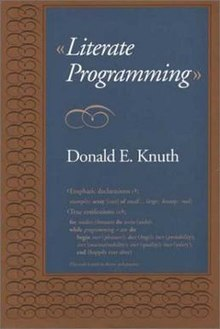
\includegraphics[width=.9\linewidth]{../images/literate-programming-book.jpg}
\label{Literate Programming Book}
\end{center}

\subsection*{Why should I care?}
\label{sec:org670397a}

Literate programming is often used in academia for reproducible research. You
can explain what your program does and your colleagues can test the program for
themselves. It's also very useful for creating tutorials.

\subsection*{Are there any other ways that literate programming could be used?}
\label{sec:org8e6a8a2}

Yes! I think it should be used in teaching. A creative teacher could use
literate programming to teach just about any subject. If properly introduced,
programming is very conducive to experimentation and play which are, in my
opinion, crucial elements of learning.

Programming can be especially useful for teaching and illustrating mathematical
concepts. Indeed, a computer is basically a mathematical sandbox.

\section*{Two Examples Of Literate Programming}
\label{sec:orgee22196}

OK, that first example was pretty boring. Thanks to the folks who made the
\href{https://threejs.org/}{Three.js} JavaScript library, and the folks at Google, we have two examples of
literate programming that are a bit more interesting.

\subsection*{Make A Spinning Cube Using Three.js}
\label{sec:orgf7cbbf1}

To make a spinning cube using the Three.js JavaScript library, we first make a
DOM element where the spinning cube will live and we include the Three.js
library.

\begin{verbatim}
<div id="cubeCanvas" class="center-perfect"></div>
<script src="https://threejs.org/build/three.js"></script>
\end{verbatim}

We then use the Three.js library to create a cute little spinning cube.

\begin{verbatim}
// Create scene and camera.
const scene = new THREE.Scene();
const camera = new THREE.PerspectiveCamera( 75, window.innerWidth / window.innerHeight, 0.1, 1000 );

// Create the renderer and set its size.
const renderer = new THREE.WebGLRenderer();
renderer.setSize( window.innerWidth / 2, window.innerHeight / 2 );

// Create our cube and add it to the scene.
const geometry = new THREE.BoxGeometry( 1, 1, 1 );
const material = new THREE.MeshBasicMaterial( { color: 0x00ff00 } );
const cube = new THREE.Mesh( geometry, material );
scene.add( cube );

// Set the camera's position.
camera.position.z = 5;

// Animate the cube.
const animate = () => {
    requestAnimationFrame( animate );
    cube.rotation.x += 0.01;
    cube.rotation.y += 0.01;
    renderer.render( scene, camera );
};

// Get the cube's canvas, add the renderer to it, and animate the cube.
window.addEventListener('DOMContentLoaded', () => {
    const cubeCanvas = document.getElementById('cubeCanvas');
    cubeCanvas.appendChild( renderer.domElement );
    animate();
});
\end{verbatim}

Look! A green spinning cube!

\subsection*{Google Colab}
\label{sec:org31b2962}

Google Colab is a popular literate programming tool for Python. Python is a very
popular programming language for data science, machine learning, and scientific
computing.

\href{https://colab.research.google.com/drive/1YUYT90gJIZ09V0YqueZnsBj2yGdYIXp0?usp=sharing}{Let's check it out!}

\section*{Other Tools For Literate Programming}
\label{sec:org9a098dc}

There are tons of other tools for literate programming, but I'll just mention a
few that I'm familiar with.

\subsection*{Honorable Mentions}
\label{sec:org06b8bda}

\begin{itemize}
\item \href{https://jupyter.org/}{Jupyter Notebook}
\item \href{https://rmarkdown.rstudio.com/}{R Markdown}
\item \href{https://www.wolfram.com/notebooks/}{Wolfram Notebooks}
\end{itemize}

\subsection*{How did you make this webpage?}
\label{sec:org8ca39e1}

I made it with \href{https://orgmode.org/}{Emacs Org-mode}.
\end{document}
